\chapter{Mengenal Kecerdasan Buatan dan Scikit-Learn}

\section{Teori}
Praktek teori penunjang yang dikerjakan :
\begin{enumerate}
\item Sejarah Perkembangan dan Definisi \textit{Artifical Intelligence}.\\ Artifical Intelligence (AI) atau sering disebut Kecerdasan Buatan, merupakan bagian dari ilmu komputer yang mempelajari bagaimana sistem kecerdasan yang ditanamkan atau ditambahkan oleh manusia ke dalam suatu teknologi yang akan dikembangkan dalam kontek ilmiah. Yang dapat melakukan atau menyelesaikan pekerjaan manusia seperti sebaik yang dilakukan manusia bahkan lebih baik\\
Awal perkembangan AI yaitu pada tahun 1950 istilah dari \textit{Artifical Intelligence} pertama kali diciptakan untuk tahap riset awal proyek AI terjadi sekitar tahun 1950 -an dengan tujuan mengeksplorasi topik penyelesaian masalah dan metode simbolik. yang mana diawali dengan kesuksesan Newell dan Simon dengan sebuah program yang disebut dengan \textit{General Problem Solver} untuk memulai penyelesaian masalah secara manusiawi. Pada tahun (1958) McCarthy dengan membuat bahasa pemrograman tingkat tinggi yang disebut  LISP yang digunakan sampai saat ini. Di tahun 1959, Nathaniel Rochester dan sebagian mahasiswanya dari IBM menciptakan sebuah program AI yang dinamakan Geometry Theorm Prover. Program ini dapat digunakan untuk menciptakan suatu teorema dengan memakai pernyataan-pernyataan yang ada. Kemudian pada tahun 1960-an Departement Pertahanan Amerika Serikat ingin mengembangkan dan melatih komputer agar memiliki penalaran seperti manusia secara mendasar. James Slagle di tahun 1963 membuat program yang mampu menyeelsaikan masalah integral. Di tahun 1968 Tom Evan membuat program yang dapat menyelesaikan analogi geometris. Pada tahun 1969-1979 Ed Feigenbaum, Bruce Buchanan dan Joshua Lederberg membuat program untuk menyelesaikan masalah molekul. Setelah itu tahun 1970-an, proyek DARPA(\textit{Defence Advanced Research Project Agency})berhasil menyelesaikan studi kasus tentang pemetaan jalan. Selanjutnya awal abad ke 21 atau lebih tepatnya pada tahun 2003, DARPA juga berhasil menciptakan asisten pribadi cerdas. Pada era undustri AI ditemukan sistem pakar (expert system) dengan nama RI yang dapat mengkonfigurasu sistem-sistem komputer baru. Pada tahun sekitar 1985 beberapa kelompok melakukan riset dan menemukan algoritma pembelajaran propagasi balik (back propagation learning) yang dapat diimplementasikan di bidang ilmu komputer. Sejak itulah kecerdesasan buatan mengalami perkembangan hingga saat ini menjadi program yang sangat kompleks dengan menerapkan algoritma dan \textit{deep learning}.

\item Definisi supervised learning, klasifikasi, regresi dan unsupervised learning. Data set, training set dan testing set
\begin{itemize}
    \item Supervised Learning dan Unsupervised Learning
    \par
    \textit{Supervised learning} merupakan ilmu yang penedekatannya mempunyai input dan output yang dapat dibuat menjadi suatu model hubungu matematis sehingga mampu melakukan prediksi dan klasifikasi berdasarkan data yang telah ada sebelumnya.  Supervised learning menggunakan data latih (data training) dalam melakukan prediksi maupun klasifikasi. Sedangkan \textit{Unsupervised Learning} yaitu tidak menggunakan label dalam memprediksi targetnya melainkan dengan melihat kesamaan dari atribut yang dimiliki. atau tidak menggunakan data latih atau data training untuk melakukan prediksi maupun klarifikasi. Jika memiliki kesamaan dari atribut atau sifat data yang diextrak maka akan dimasukkan kedalam satu kelompok(\textit{clustering}). Sehingga dapat menimbulkan banyak kelompok. Contoh penerapan metodi ini yaitu ketika seorang data analyst ingin mengelompokkan customers salah satu provider, untuk mengelompokkan customer berdasarkan kemiripan sifat tersebut tidak diperlukan data training.
    
    \item Klasifikasi dan Regresi
    \par
    Klasifikasi termasuk ke dalam supervised learning yang merupakan suatu teknik untuk  mengklasifikasikan atau menggelompokkan beberapa item item yang belum ada berlabel kedalam sebuah kelas distrit, klasifikasi mencoba mempelajari hubungan antara kumpulan variabel fitur dan variabel target. Sedangkan Regresi yaitu teknik analisis untuk mengidentifikasi suatu relasi diantara dua variabel atau lebih, sehingga dapat menemukan suatu fungsi yang memodelkan data dengan meminimalkan error atau selisih antara nilai prediksi dengan nilai sebenarnya. Regresi digunakan untuk memprediksi nilai continue. 
    
    \item Data set, Training set dan Testing set
    \par
    Data set merupakan suatu objek yang mempresentasikan sebuah data dengan relasinya pada memory. Kemudian Training set merupakan bagian dari data set yang dapat membuat algoritma yang sesuai tujuan yang diinginkan. Testing set yaitu bagian dari data set yang memiliki tujuan untuk melihat keakuratan dari data yang di tes.
\end{itemize}
\end{enumerate}

\section{Instalasi}
\begin{enumerate}
\item Melakukan installasi pada anaconda pormt dengan perintah " pip install -U scikit-learn".
    \begin{figure}[!htbp]
    \centering
    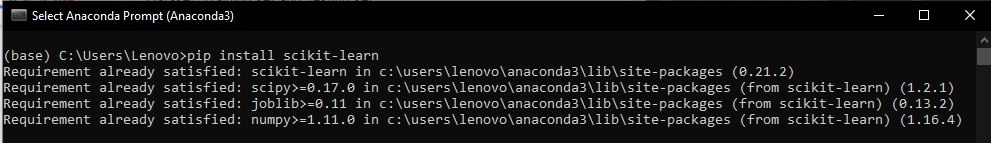
\includegraphics[scale=0.4]{figures/instalasi.jpeg}
    \end{figure}
    \newpage
    \item Setelah itu masuk ke link website yang telah diberikan yaitu "https://scikit-learn.org/stable/tutorial/basic/tutorial.html".
    \begin{lstlisting}[language=Python]
from sklearn.linear_model import LogisticRegression
from sklearn import set_config


lr = LogisticRegression(penalty='l1')
print('Default representation:')
print(lr)
# LogisticRegression(C=1.0, class_weight=None, dual=False, fit_intercept=True,
#                    intercept_scaling=1, l1_ratio=None, max_iter=100,
#                    multi_class='auto', n_jobs=None, penalty='l1',
#                    random_state=None, solver='warn', tol=0.0001, verbose=0,
#                    warm_start=False)

set_config(print_changed_only=True)
print('\nWith changed_only option:')
print(lr)
# LogisticRegression(penalty='l1')
\end{lstlisting}
\item Mencoba Loading example dataset
 \begin{lstlisting}[language=Python]
from sklearn import datasets #mengimport class dataset dari scikit learn library
iris = datasets.load_iris() #memuat dan memasukkan dataset iris ke variabel bernama iris
digits = datasets.load_digits() #membuat dan memasukkan dataset digits ke variabel digits

print(digits.data) #memberikan akses ke fitur yang dapat digunakan untuk mengklasifikasikan  sampel digit dan menampilkan diconsole

digits.target #memberikan informasi tentang data yang berhubungan atau juga dapat dijadikan sebagai label

digits.images[0] #Data selalu berupa array 2D, shape (n.samples, n.features), meskipun data aslinya mungkin memiliki bentuk yang berbeda.
\end{lstlisting}
\item Mencoba Learning and predicting
\begin{lstlisting}[language=Python]
from sklearn import svm #perintah untuk mengimport class svm dari package sklearn

digits = datasets.load_digits()    #memasukkan dan memuat dataset digits ke variabel digits

clf = svm.SVC(gamma=0.001, C=100.) #elf sebagai estimator/parameter, svm.SVC sebagai class, gamma sebagai parameter untuk menerapkan nilai secara manual

clf.fit(digits.data[:-1], digits.target[:-1]) #elf sebagai estimator/parameter, fit sebagai metode, digits.data sebagai item,[:-1] sebagai syntax python dan menampilkan outputnya


print(clf.predict(digits.data[-1:])) #predict sebagai metode lainnya, digit.data sebagai item menampilkan outputnya
\end{lstlisting}
\item Mencoba Model Persistence
\begin{lstlisting}[language=Python]
from sklearn import svm #mengimport class svm dari scikit learn library
from sklearn import datasets #mengimport class dataset dari scikit learn library
 
clf = svm.SVC(gamma=0.001, C=100.) #memanggil class SVC dan menset argument constructor SVC serta ditampung di variabel clf
X, y= datasets.load_iris(return_X_y=True) #meload datasets iris dan ditampung di variabel x untuk data sedangkan y untuk target

clf.fit(X, y) #memanggil method fit untuk melakukan training data dengan argumen data dan target dari database iris 

import pickle #mengimport pickle (agar dapat terbaca)
s = pickle.dumps(clf) #memanggil method dumps dengan argumen clf dan ditampung pada valiabel s
clf2 = pickle.loads(s) #memanggil method loads dengan argumen s dan ditampung di variabel clf2
clf2.predict(X[0:1]) #menampilkan hasil dari method predict dengan argumen data variabel x 

from joblib import dump, load #mengimport dump dan load dari library joblib
dump(clf, '1184039.joblib') #memanggil method dumps dengan argumen clf dari nama file joblib
clf3 = load('1184039.joblib') #memanggil method load dengan argumen nama file joblibnya
print(clf3.predict(X[0:1])) #menampilkan hasil dari method predict dengan argumen data variabel
\end{lstlisting}
\item Mencoba Conventions
\begin{lstlisting}[language=Python]
#Type casting
import numpy as np
from sklearn import random_projection

rng = np.random.RandomState(0)
X = rng.rand(10, 2000)
X = np.array(X, dtype='float32')
print(X.dtype)


transformer = random_projection.GaussianRandomProjection()
X_new = transformer.fit_transform(X)
print(X_new.dtype)

from sklearn import datasets
from sklearn.svm import SVC
iris = datasets.load_iris()
clf = SVC(gamma=0.001, C=100.)
clf.fit(iris.data, iris.target)
print(list(clf.predict(iris.data[:3])))
clf.fit(iris.data, iris.target_names[iris.target])
print(list(clf.predict(iris.data[:3])))

#refitting and updating parameters
import numpy as np
from sklearn.datasets import load_iris
from sklearn.svm import SVC
X, y = load_iris(return_X_y=True)
clf = SVC(gamma=0.001, C=100.)
clf.set_params(kernel='linear').fit(X, y)
clf.set_params(kernel='rbf').fit(X, y)
print(clf.predict(X[:5]))

#multiclass vs multilabel fitting
from sklearn.svm import SVC
from sklearn.multiclass import OneVsRestClassifier
from sklearn.preprocessing import LabelBinarizer

X = [[1, 2], [2, 4], [4, 5], [3, 2], [3, 1]]
y = [0, 0, 1, 1, 2]

classif = OneVsRestClassifier(estimator=SVC(random_state=0, gamma=0.001, C=100.))
print(classif.fit(X, y).predict(X))
y = LabelBinarizer().fit_transform(y)
print(classif.fit(X, y).predict(X))

from sklearn.preprocessing import MultiLabelBinarizer
y = [[0, 1], [0, 2], [1, 3], [0, 2, 3], [2, 4]]
y = MultiLabelBinarizer().fit_transform(y)
print(classif.fit(X, y).predict(X))

\end{lstlisting}
\end{enumerate}


\section{Penanganan Error}
\begin{enumerate}

\item Screenshoot Error
\begin{figure}[!htbp]
    \centering
    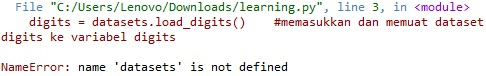
\includegraphics[scale=0.8]{figures/error.jpeg}
    \end{figure}
\item Tuliskan kode error dan jenis error
\par 
NameError: name 'datasets' is not defined
\item Solusi dari error tersebut
\par 
Python mengetahui tujuan dari nama tertentu (seperti nama fungsi bawaan seperti print ). Nama lain didefinisikan dalam program (seperti variabel). Jika Python menemukan nama yang tidak dikenali, maka mungkin akan mendapatkan kesalahan seperti diatas
Beberapa penyebab umum kesalahan ini meliputi:
\begin{enumerate}
\item Lupa memberi nilai variabel sebelum menggunakannya di pernyataan lain
\item Salah mengeja nama fungsi bawaan (mis., Mengetik "inpit" alih-alih "input")
\end{enumerate}
\end{enumerate}


